%%=============================================================================
%% Conclusie
%%=============================================================================

\chapter{Conclusie}
\label{ch:conclusie}

% TODO: Trek een duidelijke conclusie, in de vorm van een antwoord op de
% onderzoeksvra(a)g(en). Wat was jouw bijdrage aan het onderzoeksdomein en
% hoe biedt dit meerwaarde aan het vakgebied/doelgroep? 
% Reflecteer kritisch over het resultaat. In Engelse teksten wordt deze sectie
% ``Discussion'' genoemd. Had je deze uitkomst verwacht? Zijn er zaken die nog
% niet duidelijk zijn?
% Heeft het onderzoek geleid tot nieuwe vragen die uitnodigen tot verder 
%onderzoek?

\begin{table}[h]
    \centering
    \addtolength{\leftskip} {-2cm}
    \addtolength{\rightskip}{-2cm}
    \begin{tabular}{llllll}
        \hline
                                                    & \textbf{VS Code} & \textbf{Visual Studio} & \textbf{Eclipse} & \textbf{Notepad++} & \textbf{IntelliJ} \\
        \hline
        \textbf{Gemiddelde opstarttijd (in ms) }   & 2026.75          & 32025.4                & 12964.1          & 2200               & 14828.5           \\
        \textbf{Gemiddelde zoektijd (in ms) }      & 297.35           & 8.51                   & 384.97           & 6800.47            & 1452.10           \\
        \textbf{Gemiddelde build tijd C\# (in ms) } & 22285            & 46474                  & 59524.9          & NA                 & NA                \\
        \textbf{Gemiddeld CPU gebruik (in \%) }     & 0.23             & 0.00                   & 0.01             & 0.00               & 0.01              \\
        \textbf{Gemiddeld RAM gebruik (in MB) }     & 799.76           & 1321.44                & 1375.34          & 126.45             & 1465.28           \\
        \hline
    \end{tabular}
    \caption{Samenvatting van alle resultaten}
    \label{tab:resultatenCombined}
\end{table}

Als conclusie van dit onderzoek kan er genomen worden dat in algemene opzichten VS Code de meest performantie IDE is. Dit komt door de snelste opstarttijd, een snelle zoekfunctie, de snelste build tijd voor C\# code en een niet te hoog RAM gebruik. Een tweede voordeel van VS Code is dat het zeer uitbreidbaar is en niet gelimiteerd tot een specifieke programmeertaal. Een laatste voordeel van met VS Code te werken is dat het gratis is. Dit is zeker  welkom voor de beginnende ontwikkelaar, omdat dit de toetredingsdrempel tot software ontwikkeling verlaagd. Deze conclusie bied mogelijks ook een deel van de verklaring waarom VS Code momenteel de meest populaire IDE is.

Als de gebruiker meer nood heeft aan een gespecialiseerde IDE toegelegd op een specifieke taal (Java of C\#) is IntelliJ of Visual Studio ook een goede keuze. Dit komt omdat deze IDEs meer functies hebben die gebruikt kunnen worden bij het ontwikkelingsproces, dit komt dan wel met een tragere opstarttijd en meer RAM gebruik.

Notepad++ kan een goede keuze zijn als de gebruiker een programma nodig heeft met minimale functionaliteit. Hierbij kan er dan voordeel gemaakt worden van de snelle opstart en extreem lage RAM verbruik, dit kan vooral handig zijn op machines met mindere specificaties. En nadeel van deze editor is dan wel de trage zoektijd. Hiervoor kan er dan best gebruik gemaakt worden van een externe tool voor het zoeken in bestanden, zeker in grote projecten. Mogelijkheden hiervoor zijn Astrogrep\footnote{http://astrogrep.sourceforge.net/} en TextCrawler\footnote{https://www.digitalvolcano.co.uk/textcrawler.html}.

Er werd ook opgemerkt dat de prestaties van de IDE grotendeels onafhankelijk zijn van de taal waarin het project geschreven is en de performantie meer afhankelijk is van de grootte van het project. In sommige gevallen was er wel een verschil in RAM geheugen merkbaar tussen de twee projecten, maar deze verhoging was niet consistent over verschillende IDEs heen.

Tot slot is er in dit onderzoek opgemerkt dat de tijd dat een C\# project nodig heeft om te builden afhangt van de IDE die het build commando uitvoert. Dit werd niet verwacht aangezien deze onderliggend hetzelfde commando gebruiken, meer bepaald het dotnet build commando. Hier is meer onderzoek voor nodig om te bepalen waarom dit zo is.

\begin{figure}[h]
    \centering
    \addtolength{\leftskip} {-2cm}
    \addtolength{\rightskip}{-2cm}
    \begin{minipage}{0.6\linewidth}
        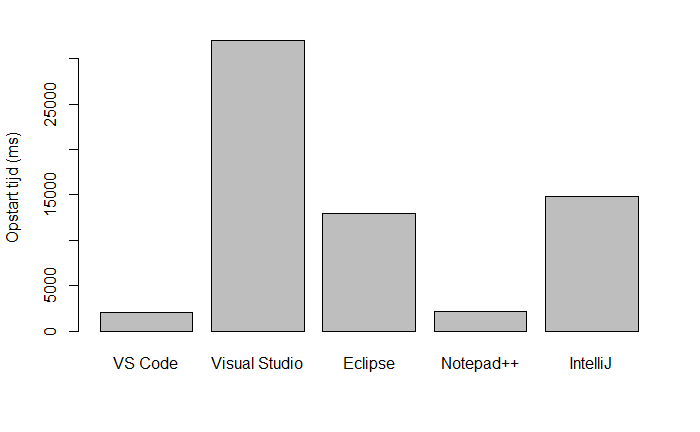
\includegraphics[width=1\linewidth]{StartupTime.png}
        \vspace*{-1.4cm}
        \caption{Gemiddelde opstarttijd}
        \label{fig:startupTime}
    \end{minipage}%
    \begin{minipage}{0.6\linewidth}
        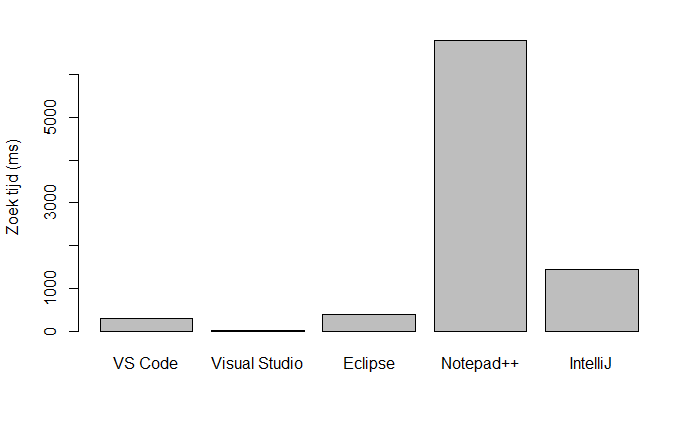
\includegraphics[width=1\linewidth]{SearchTime.png}
        \vspace*{-1.4cm}
        \caption{Gemiddelde zoektijd}
        \label{fig:searchTime}
    \end{minipage}
\end{figure}

\begin{figure}[h]
    \centering
    \addtolength{\leftskip} {-2cm}
    \addtolength{\rightskip}{-2cm}
    \begin{minipage}{0.6\linewidth}
        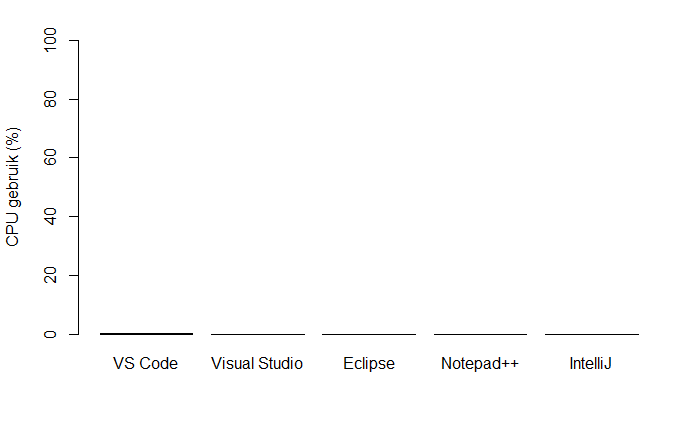
\includegraphics[width=1\linewidth]{CPUUsage.png}
        \vspace*{-1.4cm}
        \caption{Gemiddeld CPU gebruik}
        \label{fig:CPUUsage}
    \end{minipage}%
    \begin{minipage}{0.6\linewidth}
        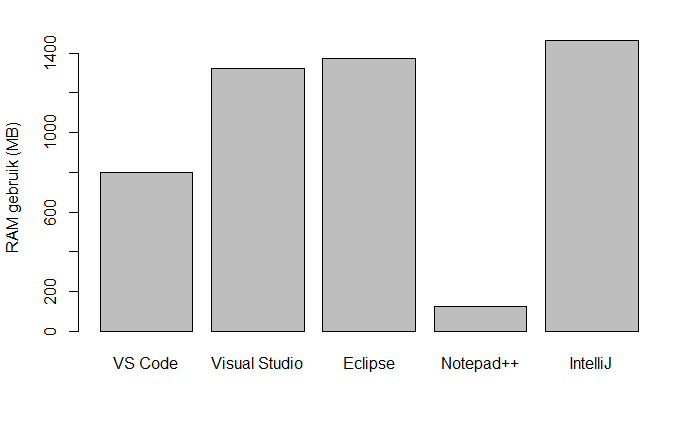
\includegraphics[width=1\linewidth]{RAMUsage.png}
        \vspace*{-1.4cm}
        \caption{Gemiddelde RAM gebruik}
        \label{fig:RAMUsage}
    \end{minipage}
\end{figure}

\begin{figure}[h!]
    \centering
    \begin{minipage}{0.6\linewidth}
        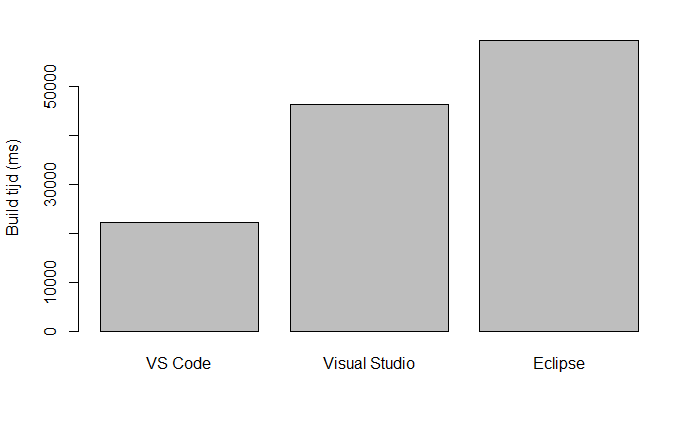
\includegraphics[width=1\linewidth]{BuildTime.png}
        \vspace*{-1.4cm}
        \caption{Gemiddelde build tijd}
        \label{fig:buildTime}
    \end{minipage}%
\end{figure}
